\part{Impresa e organizzazione aziendale}
\chapter{Impresa}
Un’impresa può essere analizzata attraverso tre principali prospettive:\index{Impresa!fenomeno}
\begin{enumerate}
    \item \textit{Fenomeno soggettivo:} Quando parliamo dell'impresa come fenomeno soggettivo, ci riferiamo al ruolo delle persone e delle relazioni umane all'interno dell’organizzazione. Il focus è sull'integrazione dei lavoratori e sull'interdipendenza tra gli obiettivi dell'impresa e quelli dei soggetti che la compongono.
    \item \textit{Fenomeno oggettivo:} L’approccio oggettivo vede l’impresa come un’entità razionale, de-personalizzata, dove l’efficienza è la priorità assoluta. Si tratta di un modello in cui si cerca di raggiungere la massimizzazione del risultato utilizzando il minimo delle risorse, ignorando elementi immateriali che non sono misurabili in termini puramente economici.
    \item \textit{Fenomeno interattivo:} In questa prospettiva, l'impresa è vista come un sistema aperto, che interagisce con l'ambiente circostante. Una parte delle relazioni dell'impresa può essere oggettivamente quantificabile, ma vi sono anche elementi non economici, difficilmente controllabili, che influiscono sulla sua gestione. Qui l’impresa è intesa come un'entità viva che influenza e viene influenzata dal sistema più vasto in cui opera.
\end{enumerate}

Per analizzare l’impresa sono stati sviluppati diversi approcci teorici:\index{Impresa!approccio}
\begin{itemize}
    \item L'\textit{approccio riduzionistico-analitico} è stato storicamente adottato dalle teorie classiche, come quelle di Frederick Taylor. Esso scompone l'impresa in parti più piccole per studiare come funzionano singolarmente, con l’obiettivo di migliorare l’efficienza complessiva.
    \item L'\textit{approccio evolutivo} invece guarda al fenomeno dell'impresa nel suo insieme, osservando come le sue componenti si evolvono nel tempo. Questo approccio riconosce che l'impresa non è statica, ma cambia continuamente in risposta all'ambiente.
    \item L'\textit{approccio sistemico}, infine, si concentra sullo studio delle relazioni tra le varie componenti di un fenomeno. Vede l’impresa come parte di un sistema più ampio e considera come i diversi elementi interagiscono tra loro e con altri sistemi.
\end{itemize}

\section{Approccio sistemico}
Un sistema non è solo una raccolta casuale di parti. È un insieme integrato in cui ogni elemento è interdipendente e tutte le componenti interagiscono per un fine comune. Questa è una caratteristica fondamentale di un sistema. Le parti non possono essere considerate isolatamente, ma devono essere comprese nel contesto delle loro relazioni reciproche.

In un’impresa, ciò significa che non possiamo studiare le singole funzioni aziendali (come produzione, marketing, finanza) separatamente senza considerare come interagiscono tra loro. Anche le relazioni dell’impresa con l’ambiente esterno – clienti, fornitori, regolatori – sono cruciali per comprenderne il funzionamento complessivo.

\begin{redbar}
Secondo la \textbf{teoria dei sistemi}, ogni impresa è parte di un sistema più ampio (un sovra-sistema) e, al suo interno, contiene a sua volta dei sottosistemi. Questa struttura multilivello è tipica di ogni sistema complesso. Un principio chiave della teoria dei sistemi è:
\begin{center}
\begin{minipage}{0.9\textwidth}
\textit{Il valore del sistema nel suo insieme è maggiore della somma dei valori delle singole parti.}
\end{minipage}
\end{center}
\end{redbar}
Questo fenomeno è noto come \textit{sinergia}\index{Impresa!sinergia}, ed è ciò che permette a un sistema ben organizzato di raggiungere risultati superiori rispetto a quelli che otterrebbe semplicemente sommando le prestazioni individuali delle sue parti.
\begin{redbar}
Un \textbf{sistema}\index{Sistema}, dunque, è un insieme complesso di elementi che dipendono l’uno dall’altro. Le parti di un sistema non solo si completano a vicenda, ma esistono relazioni chiave tra esse. L’elemento essenziale è la complementarità tra le parti, che le collega in un tutt'uno coerente.
\end{redbar}
Esistono tre tipi principali di sistemi:\index{Sistema!tipo}
\begin{enumerate}
    \item \textit{Sistemi chiusi:} non scambiano né energia né informazioni con l’ambiente esterno. Sono isolati dal contesto esterno e operano in modo autonomo.
    \item \textit{Sistemi aperti:} interagiscono liberamente con l’ambiente esterno, ricevendo input e generando output.
    \item \textit{Sistemi parzialmente aperti:} hanno una chiusura operazionale, ossia una barriera che controlla l’ingresso e l’uscita di energia, materia o informazioni. Un’impresa è un esempio di sistema parzialmente aperto, in quanto regola le sue interazioni con l’esterno in base alle sue esigenze e obiettivi.
\end{enumerate}
Ad esempio, un’azienda può essere vista come un sistema aperto: essa riceve input dall’ambiente esterno (materie prime, persone, informazioni, risorse finanziarie), trasforma tali input, e produce output sotto forma di prodotti e servizi.

Un sistema ha una determinata \textit{capacità}\index{Sistema!capacità}, ovvero la potenzialità di rapportarsi con l’esterno in base alla sua struttura. Tuttavia, è l’organo di governo del sistema a decidere in che misura sfruttare questa capacità. Il \textit{grado di apertura}\index{Sistema!grado di apertura} è dunque una scelta strategica che determina il livello di interazione del sistema con l’ambiente esterno. Un’impresa, ad esempio, può scegliere di aprirsi a nuovi mercati o di chiudersi in un regime di autarchia.

Le relazioni tra le parti di un sistema possono avvenire all’interno dello stesso sistema (intra-sistemiche)\index{Sistema!Relazione!intra-sistemiche} o tra sistemi diversi (inter-sistemiche)\index{Sistema!Relazione!inter-sistemiche}. È essenziale comprendere queste interazioni, poiché spesso le connessioni logiche si trasformano in interazioni fisiche, tecniche ed economiche. Un sistema non è isolato, ma partecipa a un insieme più ampio di sovrasistemi e sottosistemi.

\begin{figure}[ht]
    \centering
    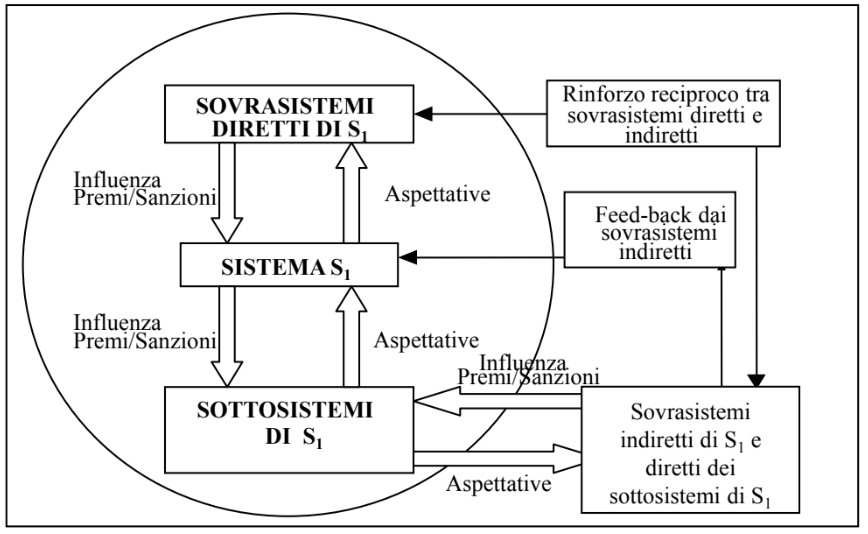
\includegraphics[width=0.6\linewidth]{images/sovra-sistemi.PNG}
    \caption{Sovra-sistemi e sotto-sistemi}
    \label{fig:sovra-sistemi}
\end{figure}

La \textit{consonanza}\index{Sistema!Relazione!consonanza} tra sistemi si verifica quando essi sono strutturalmente compatibili e possono cooperare in maniera efficace. La \textit{risonanza}\index{Sistema!Relazione!risonanza}, invece, rappresenta il massimo grado di consonanza, un livello ideale in cui le interazioni tra i sistemi creano armonia e sviluppano ulteriormente l’efficacia delle relazioni. Un esempio utile è la metafora dell’orchestra, dove i singoli strumenti (sistemi) devono essere accordati (consonanza) e suonare insieme armoniosamente (risonanza) per creare una melodia coerente.

\begin{figure}[ht]
    \centering
    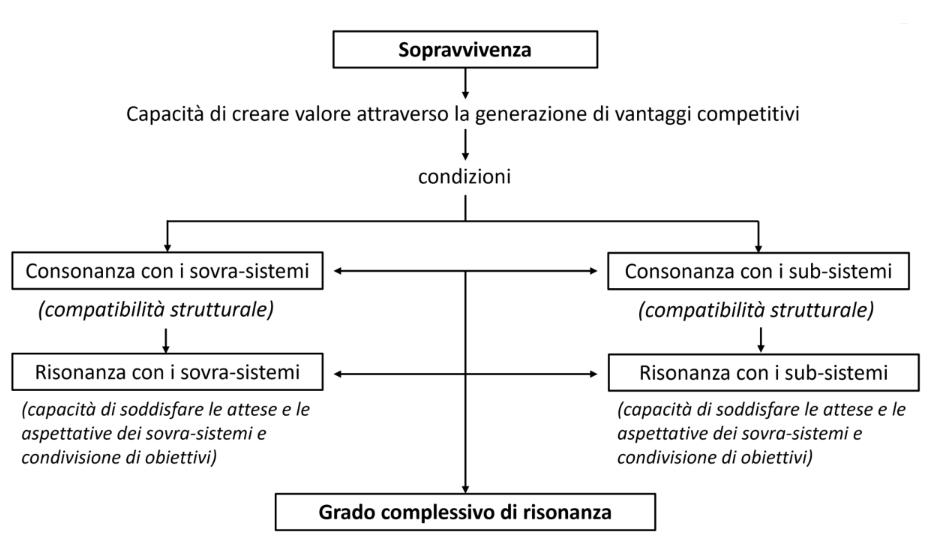
\includegraphics[width=0.6\linewidth]{images/consonanza-risonanza.PNG}
    \caption{Consonanza e risonanza}
    \label{fig:consonanza-risonanza}
\end{figure}

\section{Struttura di un sistema impresa}
La struttura di un sistema è composta da elementi a cui sono assegnati ruoli, attività e compiti specifici. Ogni sistema ha due componenti fondamentali:\index{Sistema!struttura}
\begin{enumerate}
    \item Una \textit{struttura logica:} si riferisce all'insieme delle regole e delle relazioni che determinano il funzionamento del sistema.
    \item Una \textit{struttura fisica}: include gli elementi materiali o tangibili del sistema.
\end{enumerate}

\begin{Example}{Struttura logica e fisica}{}
\begin{itemize}
    \item Consideriamo, per esempio, una pizzeria: la sua struttura logica comprende il menù, i processi di preparazione e le relazioni con i clienti. La struttura fisica, invece, riguarda il layout del locale, le attrezzature e il personale.
    \item Lo stesso concetto si applica a una banca. La sua struttura logica riguarda i servizi offerti (conti correnti, prestiti), i processi interni e la gestione del rischio, mentre la struttura fisica include le filiali, gli sportelli automatici e gli uffici.
\end{itemize}
\end{Example}
Un sistema non nasce già formato, ma attraversa diverse fasi di sviluppo. Si parte dall'idea imprenditoriale, che definisce lo schema organizzativo di massima, poi si passa all’emersione di una struttura logica e, infine, alla sua concretizzazione in una struttura fisica. Man mano che il sistema evolve, si definiscono le relazioni tra le varie parti, e il sistema nel suo complesso prende vita.
Le decisioni prese in queste fasi possono essere suddivise in preliminari (scelta delle componenti strutturali), di governo (gestione delle relazioni) e operative (utilizzo della struttura).

\begin{figure}[ht]
    \centering
    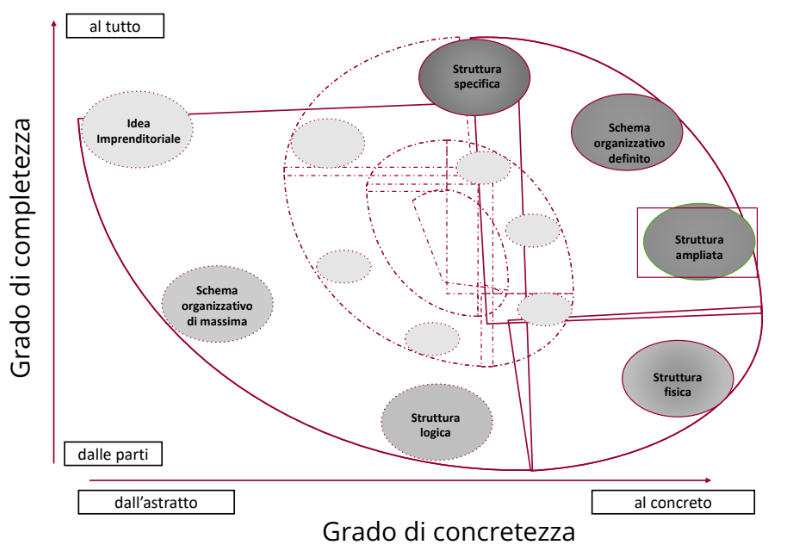
\includegraphics[width=0.7\linewidth]{images/emersione-sistema-impresa.PNG}
    \caption{Emersione del sistema impresa}
    \label{fig:emersione-sistema-impresa}
\end{figure}
Ogni sistema ha bisogno di un "cervello" che ne regoli il funzionamento. Nell'impresa, questo ruolo è svolto dall'\textit{organo di governo}\index{Impresa!organo di governo}, che si occupa di filtrare le pressioni interne ed esterne, identificando obiettivi comuni e regolando le relazioni tra le parti del sistema. Questo organo è essenziale per mantenere l'equilibrio e garantire che il sistema possa evolvere in modo armonioso.

\begin{redbar}
L’\textbf{impresa}\index{Impresa} può essere descritta come un sistema dinamico che interagisce costantemente con l’ambiente esterno.    
\end{redbar}
Per essere considerato un sistema, l’insieme aziendale deve soddisfare tre condizioni fondamentali. Innanzitutto, deve essere costituito da una pluralità di elementi distinti, che formano l'ossatura del sistema. Questi elementi, poi, devono essere interconnessi attraverso relazioni e canali di comunicazione, consentendo lo scambio di informazioni e risorse tra le varie parti. Infine, l’interazione tra le parti del sistema deve essere orientata al raggiungimento di un obiettivo comune, il che implica una finalità condivisa che guida l'intero meccanismo organizzativo verso il successo aziendale.

Le caratteristiche chiave del sistema impresa si sviluppano attorno a quattro concetti fondamentali:
\begin{enumerate}
    \item \textit{Entropia negativa}.\index{Impresa!Caratteristiche!entropia negativa} Il concetto di entropia deriva dalla fisica e si riferisce alla tendenza naturale verso il disordine. In un sistema aziendale, l’entropia negativa rappresenta la capacità di resistere a questa tendenza. Un’impresa, infatti, deve continuamente organizzarsi per evitare il caos che potrebbe derivare da disconnessioni tra le sue parti, perdite di risorse o inefficienze.
    \item \textit{Equifinalità}.\index{Impresa!Caratteristiche!equifinalità} Nei sistemi aperti, come le imprese, uno stesso obiettivo può essere raggiunto attraverso percorsi diversi, partendo da condizioni iniziali differenti. Questo significa che non esiste una sola "best way" per il successo: le imprese possono adottare strategie diverse, in base al loro contesto e alle loro risorse, pur raggiungendo risultati simili. 
    \item \textit{Trasformazione}.\index{Impresa!Caratteristiche!trasformazione} Il sistema impresa può essere visto come un processo di trasformazione continuo. Gli elementi provenienti dall’esterno, come materie prime, risorse umane e informazioni, entrano nel sistema come input. Questi input vengono trasformati attraverso processi interni, che possono essere fisici, tecnici o concettuali, per poi essere restituiti all’esterno come output. Gli output, che possono assumere la forma di prodotti o servizi, rappresentano il risultato del lavoro dell'impresa e costituiscono la sua principale fonte di valore.
    \item \textit{Omeostasi}.\index{Impresa!Caratteristiche!omeostasi} Per sopravvivere e prosperare, un’impresa deve essere in grado di mantenere un equilibrio dinamico tra le sue componenti interne e l’ambiente esterno. Questo meccanismo di regolazione, noto come omeostasi, consente all’impresa di adattarsi ai cambiamenti, regolando automaticamente le sue operazioni per mantenere l’equilibrio.
\end{enumerate}
Per garantire la sopravvivenza, l’impresa deve mantenere l’entropia interna compatibile con quella dell’ambiente esterno. In pratica, deve adattarsi costantemente ai cambiamenti e alle esigenze del contesto in cui opera.

Le risorse di un'impresa si dividono in due grandi categorie:\index{Impresa!risorse} materiali e immateriali. Le risorse materiali includono elementi fisici come attrezzature, edifici e capitali finanziari, mentre le risorse immateriali comprendono fattori intangibili, come le conoscenze e le relazioni con i clienti o partner. Tra queste, le risorse immateriali sono spesso considerate i veri fattori critici di successo. Le risorse conoscitive, ad esempio, rappresentano il patrimonio di know-how e competenze accumulate dall’impresa, mentre le risorse relazionali riflettono la sua capacità di costruire e mantenere rapporti di fiducia con gli stakeholder.

\section{Tipologie di sistema impresa}
L’impresa è un sistema complesso che può essere visto come:
\begin{itemize}
    \item \textit{Sociale:} interagisce con persone e comunità.
    \item \textit{Economico:} genera valore e profitti.
    \item \textit{Tecnico:} utilizza tecnologie e strutture operative.
    \item \textit{Aperto:} interagisce con l’ambiente esterno, ma con confini ben definiti.
    \item \textit{Autopoietico:} si autoregola per sopravvivere e crescere.
    \item \textit{Relazionale e cognitivo:} costruisce legami e acquisisce conoscenze per evolvere.
\end{itemize}
McKinsey propone un modello basato su sette elementi per valutare la capacità di un’impresa di attuare una strategia\index{Impresa!7s}:
\begin{enumerate}
    \item \textit{Strategia:} il piano per costruire un vantaggio competitivo.
    \item \textit{Struttura:} l’organizzazione interna, spesso gerarchica o decentralizzata.
    \item \textit{Sistemi:} i processi aziendali quotidiani.
    \item \textit{Shared values:} i valori condivisi che definiscono la cultura aziendale.
    \item \textit{Stile:} il modo in cui la leadership aziendale influenza l’organizzazione.
    \item \textit{Staff:} la forza lavoro e le sue competenze.
    \item \textit{Skills:} le capacità del personale.
\end{enumerate}

\subsection{Ambiente d'impresa}
L’ambiente esterno\index{Impresa!ambiente} rappresenta tutto ciò che può influenzare, direttamente o indirettamente, la sopravvivenza e la crescita dell’impresa. Da una parte, l’ambiente fornisce le regole del gioco, sotto forma di normative e vincoli. Dall’altra, è anche una fonte di minacce e opportunità che possono plasmare il futuro dell’azienda. 

Il rapporto tra l’impresa e l’ambiente si sviluppa su più livelli. 
\begin{enumerate}
    \item \textit{Livello competitivo:} riguarda le relazioni concorrenziali o cooperative con altre aziende.
    \item \textit{Livello socio-culturale:} include elementi come i valori, le norme sociali, le infrastrutture e le istituzioni che regolano il contesto in cui l’impresa opera.
    \item \textit{Livello fisico-naturale:} si riferisce all'ambiente naturale e alle risorse ecologiche. 
\end{enumerate}
Le imprese moderne non possono più limitarsi ad adeguarsi passivamente alle condizioni esterne, ma devono sviluppare una capacità proattiva per anticipare i cambiamenti. Si parla quindi di morfogenesi, cioè della capacità dell'impresa di trasformarsi continuamente per adattarsi all'ambiente in evoluzione.

L’ambiente in cui operano le imprese moderne è caratterizzato da un alto grado di incertezza e complessità. L’incertezza si riferisce alla difficoltà di prevedere con esattezza gli sviluppi futuri, mentre la complessità riguarda la varietà degli attori e dei fattori in gioco, che interagiscono su più livelli. Negli ultimi anni, infatti, abbiamo assistito a una serie di eventi straordinari che hanno trasformato profondamente il contesto economico, sociale e tecnologico in cui operano le imprese. La pandemia di Covid-19 e il conflitto russo-ucraino, ad esempio, hanno avuto un impatto devastante sulle economie globali, creando incertezze e destabilizzando interi settori produttivi. In parallelo, lo sviluppo tecnologico continua a evolversi a ritmi sempre più accelerati. Tecnologie come l’intelligenza artificiale, l’automazione e l’Internet of things stanno ridefinendo i modelli di produzione e distribuzione.

L’\textit{internazionalizzazione}\index{Impresa!internazionalizzazione} rappresenta il processo attraverso cui le imprese si aprono a nuovi mercati esteri, instaurando rapporti commerciali e produttivi con altre aziende e istituzioni. Questa apertura si declina in due forme principali: una forma leggera, caratterizzata da semplici attività di esportazione, e una forma pesante, che implica il trasferimento di risorse produttive all’estero.

La \textit{globalizzazione}\index{Impresa!globalizzazione}, d’altro canto, si riferisce al fenomeno di unificazione dei mercati su scala mondiale, favorito dall’innovazione tecnologica. Questo processo ha portato a una progressiva omogeneizzazione dei consumi e dei bisogni dei clienti in tutto il mondo, spingendo le imprese a sfruttare economie di scala e ad adottare strategie più globalizzate. 

L’aumento della concorrenza a livello globale ha spinto le imprese a concentrarsi sulle proprie competenze chiave, sviluppando strategie per affrontare una competizione sempre più aggressiva e ipercompetitiva. In un contesto caratterizzato da continue trasformazioni, le imprese devono mantenere flessibilità, innovazione e capacità di integrazione tra le varie parti del sistema. Solo attraverso un’attenta gestione delle risorse e una costante attenzione all’ambiente esterno, le imprese possono garantire la propria sopravvivenza e crescita a lungo termine.